\documentclass[tikz,border=3pt]{standalone}
\usepackage[utf8]{inputenc}
\usepackage[T1]{fontenc}
\usepackage{lmodern}
\renewcommand{\familydefault}{\sfdefault}
\usepackage{sansmath}\sansmath
\usepackage{chemfig}
\usepackage{pgfplots}\pgfplotsset{compat=1.18,/pgf/number format/use comma,/pgf/number format/1000 sep={.}}
\usetikzlibrary{arrows.meta,calc,positioning,decorations.pathmorphing,patterns}
% paleta del sitio
\definecolor{nar}{HTML}{E8680C}\definecolor{narc}{HTML}{FFB35C}\definecolor{hielo}{HTML}{FFF3E8}
\definecolor{tinta}{HTML}{1D1D1F}\definecolor{gris}{HTML}{6E6E73}\definecolor{lila}{HTML}{7C5CF0}
\definecolor{azul}{HTML}{2F6FD6}\definecolor{menta}{HTML}{17A673}\definecolor{coral}{HTML}{E8342A}
\begin{document}
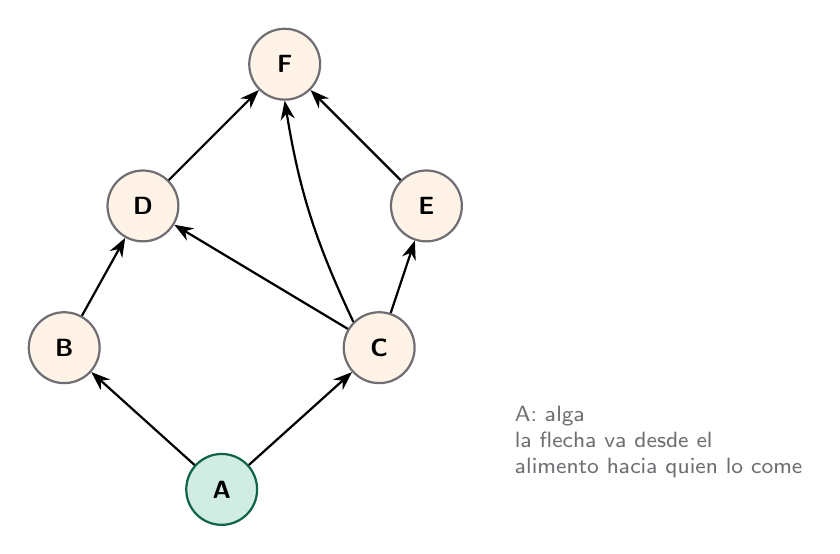
\begin{tikzpicture}[font=\small,>={Stealth[length=2.4mm]}]
\tikzset{esp/.style={circle,draw=gris,fill=hielo,thick,minimum size=0.9cm,font=\small\bfseries}}
\node[esp,fill=menta!20,draw=menta!60!black] (A) at (2,0) {A};
\node[esp] (B) at (0,1.8) {B};
\node[esp] (C) at (4,1.8) {C};
\node[esp] (D) at (1,3.6) {D};
\node[esp] (E) at (4.6,3.6) {E};
\node[esp] (F) at (2.8,5.4) {F};
\draw[->,thick] (A) -- (B); \draw[->,thick] (A) -- (C);
\draw[->,thick] (B) -- (D); \draw[->,thick] (C) -- (D); \draw[->,thick] (C) -- (E);
\draw[->,thick] (D) -- (F); \draw[->,thick] (E) -- (F);
\draw[->,thick] (C.north west) to[bend left=8] (F.south);
\node[anchor=west,text=gris,font=\footnotesize,align=left] at (5.6,0.6) {A: alga\\la flecha va desde el\\alimento hacia quien lo come};
\end{tikzpicture}
\end{document}
